\documentclass{beamer}

\usepackage[utf8]{inputenc}

\usepackage{tgbonum}

\usepackage{utopia} %font utopia imported
\usepackage{xeCJK} % 导入中文支持

\usetheme{Madrid}
\usecolortheme{default}

%------------------------------------------------------------
%This block of code defines the information to appear in the
%Title page
\title[Top/Down] %optional
{Consensus Problems in Networks of Agents\\ with Switching Topology and Time-Delays}

% \subtitle{}

\author[JC] % (optional)
{赵继超}

% \institute[VFU] % (optional)
% {
%     \inst{1}%
%     Faculty of Physics\\
%     Very Famous University
%     \and
%     \inst{2}%
%     Faculty of Chemistry\\
%     Very Famous University
% }

\date[\today] % (optional)
{分享暨个人总结}

% \logo{\includegraphics[height=1.5cm]{lion-logo.jpg}}

%End of title page configuration block
%------------------------------------------------------------



%------------------------------------------------------------
%The next block of commands puts the table of contents at the 
%beginning of each section and highlights the current section:

\AtBeginSection[]
{
\begin{frame}
    \frametitle{Table of Contents}
    \tableofcontents[currentsection]
\end{frame}
}
%------------------------------------------------------------


\begin{document}

%The next statement creates the title page.
\frame{\titlepage}


%---------------------------------------------------------
%This block of code is for the table of contents after
%the title page
\begin{frame}
\frametitle{Table of Contents}
\tableofcontents
\end{frame}
%---------------------------------------------------------


\section{Introduction}

%---------------------------------------------------------
%Changing visivility of the text
% \begin{frame}
% \frametitle{Sample frame title}
% This is a text in second frame. For the sake of showing an example.

% \begin{itemize}
%     \item<1-> $u_i = \sum_{j\in N_i}a_{ij}(x_j-x_i)$
%     \item<2-> $u_i(t) = \sum_{j\in N_i}a_{ij}[x_j(t-\tau_{ij})-x_i(t-\tau_{ij})]$
%     \item<3> Text visible on slides 3
%     \item<4-> Text visible on slide 4
% \end{itemize}
% \end{frame}

%---------------------------------------------------------


%---------------------------------------------------------
%Example of the \pause command
% \begin{frame}
% In this slide %\pause

% the text will be partially visible %\pause

% And finally everything will be there
% \end{frame}
%---------------------------------------------------------

\section{Consensus Problems}

%---------------------------------------------------------
%Two columns
\begin{frame}
    \frametitle{Some Basic Notations}
    
    \begin{columns}
    
    \column{0.5\textwidth}
    \begin{itemize}
    \item adjacency matrix
    \item neighbors nodes
    \item decision value
    \item $\chi$-Consensus Problesm
    \item Ave/Max/Min Consensus
    \end{itemize}
    
    \column{0.5\textwidth}
    \begin{itemize}
        \item $\mathcal{A}=[a_{ij}]$
        \item $N_i$
        \item $\alpha(x^*)$
        \item $\chi$
        \item Ave(x)/Max(x)/Min(x)
    \end{itemize}

    \end{columns}
    \end{frame}
%---------------------------------------------------------

\section{Consensus Protocols}

%---------------------------------------------------------
%Highlighting text
\begin{frame}
\frametitle{Model Consensus Protocols}

% 本部分主要介绍了一致性的协议。

\begin{block}{CT Model}
    $\dot{x}_i = u_i(t)$
\end{block}

\begin{alertblock}{DT Model}
    $x_i(k+1) = x_i(k) + \epsilon u_i(k), \epsilon>0$
\end{alertblock}

% \begin{examples}
% Sample text in green box. The title of the block is "Examples".
% \end{examples}

\begin{block}{A1 Zero Communication Time-Delay}
    $u_i = \sum_{j\in N_i}a_{ij}(x_j-x_i)$
\end{block}

\begin{alertblock}{A2 Communication Time-Delay $\tau_{ij}>0$}
    $u_i(t) = \sum_{j\in N_i}a_{ij}[x_j(t-\tau_{ij})-x_i(t-\tau_{ij})]$
\end{alertblock}

% 我们主要研究平均一致性问题。

\end{frame}
%---------------------------------------------------------
\begin{frame}
    \frametitle{Remark}
    Consensus Problems:

    \quad 1. Dynamic Networks 

    \quad 2. Consensus Protocols
\end{frame}

%---------------------------------------------------------
%Highlighting text
\begin{frame}
    \frametitle{Laplacians}
    
    % 本部分主要介绍了一致性的协议。
    
    \begin{block}{Laplacians}
        $l_{ij} = \left\{
            \begin{array}{ll}
                \sum_{k=1,k\ne i}^n a_{ik}, & j=i\\
                -a_{ij}, & j\ne i
            \end{array}\right.$
    \end{block}
    
    \begin{alertblock}{A1 State Evolves}
        $\dot{x}(t) = -Lx(t)$
    \end{alertblock}
    
    % \begin{examples}
    % Sample text in green box. The title of the block is "Examples".
    % \end{examples}
    
    \begin{block}{A1 State Evolves with Switchin Topology}
        $\dot{x}(t) = -L_kx(t),\ k=s(t)$
    \end{block}
    
    \begin{alertblock}{A1 DT}
        $x(k+1) = P_\epsilon x(k),\ P_\epsilon = I - \epsilon L$
    \end{alertblock}
    
    % 我们主要研究平均一致性问题。
    
    \end{frame}
%---------------------------------------------------------

\section{Algebric Graph Theory: Properties of Laplacians}

%---------------------------------------------------------
%Highlighting text
\begin{frame}
    \frametitle{Balanced Graph}
    
        Balanced Node

        $$\deg_{out}(v_i) = \deg_{in}(v_i)$$

        Balanced Graph

        $$\deg_{in}(v_i) = \sum_{j=1}^{n}a_{ji},\quad \deg_{out}(v_i) = \sum_{j=1}^{n}a_{ij}$$

        \begin{figure}[htbp]
            \centering
            % \includegraphics{}
            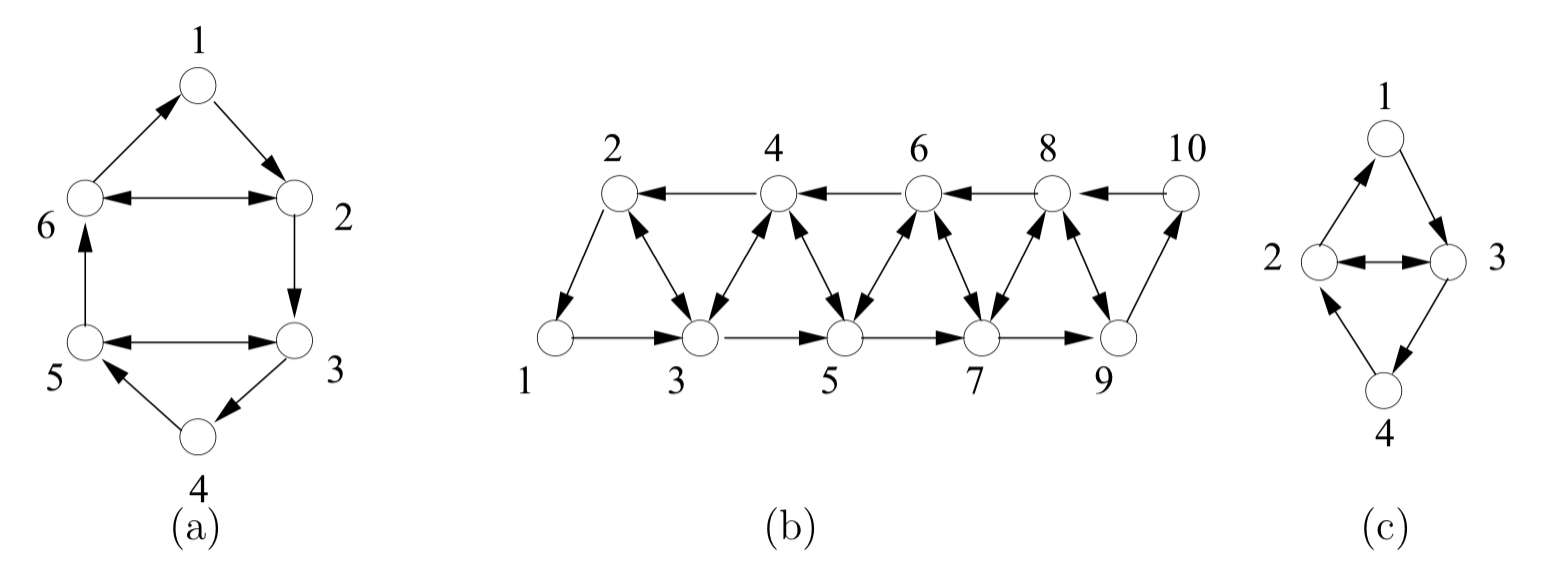
\includegraphics[width=10cm]{figures/Fig3-BalancedGraphs.jpeg}
            \label{BalancedGraphs}
            % \caption{平衡图的三个例子}
        \end{figure}
    \end{frame}
%---------------------------------------------------------
%Highlighting text
\begin{frame}
\frametitle{Laplacians}

%Example of the \pause command
    $$L = \mathcal{L}(G) = \Delta-\mathcal{A}$$ %\pause
    
    $\Delta$ (degree matrix) $\rightarrow$ diag($\deg_{out}(v_i)$) %\pause
    
    $\mathcal{A}$ (adjacency matrix) $\in$ \{0,1\}

    $w_r: \quad L w_r = \lambda w_r$
    
    $w_l: \quad w_l L = w_l \lambda$

    $SC$ (Strongly Connected)

\end{frame}
%---------------------------------------------------------

\section{A Counterexample for Average-Consensus}

%---------------------------------------------------------
%Highlighting text
\begin{frame}
\frametitle{Counterexample}
\begin{columns}
    
    \column{0.5\textwidth}
    \begin{figure}[htbp]
        \centering
        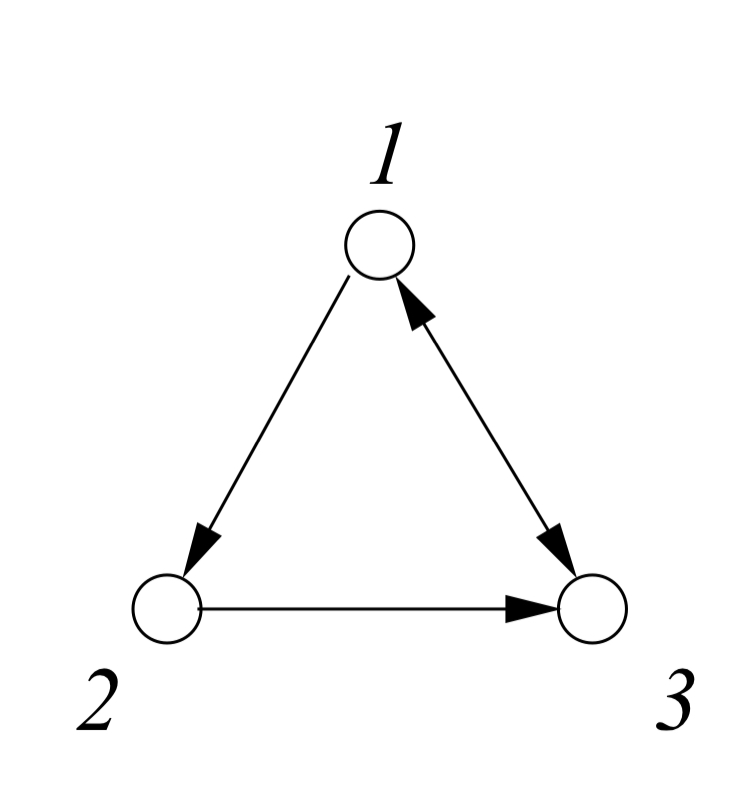
\includegraphics[width=4cm]{figures/Fig2-ConnectedDigraph.jpeg}
        \label{ConnectedDigraph}
        % \caption{一个不能使用协议(\ref{A1})解决平均一致性问题的3阶连通图}
    \end{figure}

    \begin{equation}
        \mathcal{V} = \{1, 2, 3 \},\quad \mathcal{E}=\{12, 23, 31, 13\}.
        \notag
    \end{equation}

    \column{0.5\textwidth}
    \begin{equation}
        D = \left[
        \begin{matrix}
            2 & 0 & 0 \\
            0 & 1 & 0 \\
            0 & 0 & 1 
        \end{matrix}
        \right],
        A = \left[
        \begin{matrix}
            0 & 1 & 1 \\
            0 & 0 & 1 \\
            1 & 0 & 0 
        \end{matrix}
        \right]
        \notag
    \end{equation}

    \begin{equation}
        L = \left[
        \begin{matrix}
            2 & -1 & -1 \\
            0 & 1 & -1 \\
            -1 & 0 & 1 
        \end{matrix}
        \right]
        \notag
    \end{equation}

\end{columns}
\end{frame}
%---------------------------------------------------------

\section{Networks with Fixed or Switching Topology}

%---------------------------------------------------------
%Highlighting text
\begin{frame}
\frametitle{Fixed Topology}

\begin{equation}
    x^* = \lim_{t\rightarrow +\infty}x(t) = Rx_0 = w_r(w_L^T x_0) = \frac{1}{\sqrt{n}}(w_l^Tx_0)\mathbf{1}
    \notag
\end{equation}

\end{frame}
%---------------------------------------------------------

\section{Networks with Communication Time-Delays}

%---------------------------------------------------------
%Highlighting text
\begin{frame}
\frametitle{Time-Delays}
\begin{equation}
    \dot{x}_i(t) = \sum_{j\in N_i} a_{ij} [x_j(t-\tau_{ij}) - x_i(t-\tau_{ij})].
    \notag
\end{equation}

\begin{equation}
    \tau \le \frac{\pi}{4d_{max}(G)}
    \notag
\end{equation}

\end{frame}
%---------------------------------------------------------

\section{Max-Consensus and Leader Determination}

%---------------------------------------------------------
%Highlighting text
\begin{frame}
\frametitle{Max-Consensus}

\begin{equation}
    \notag
    x_i(k+1)=max(x_i(k),u_i(k))
\end{equation}

\begin{equation}
    \notag
    x_i(k+1) = \frac{1}{2}(x_i(k)+u_i(k)+|x_i(k)-u_i(k)|) \quad u_i(k) = \max_{j\in N_i}x_j
\end{equation}

\end{frame}
%---------------------------------------------------------

\section{Simulation Results}

%---------------------------------------------------------
\begin{frame}
\frametitle{Simulation}
\begin{figure}[htbp]
    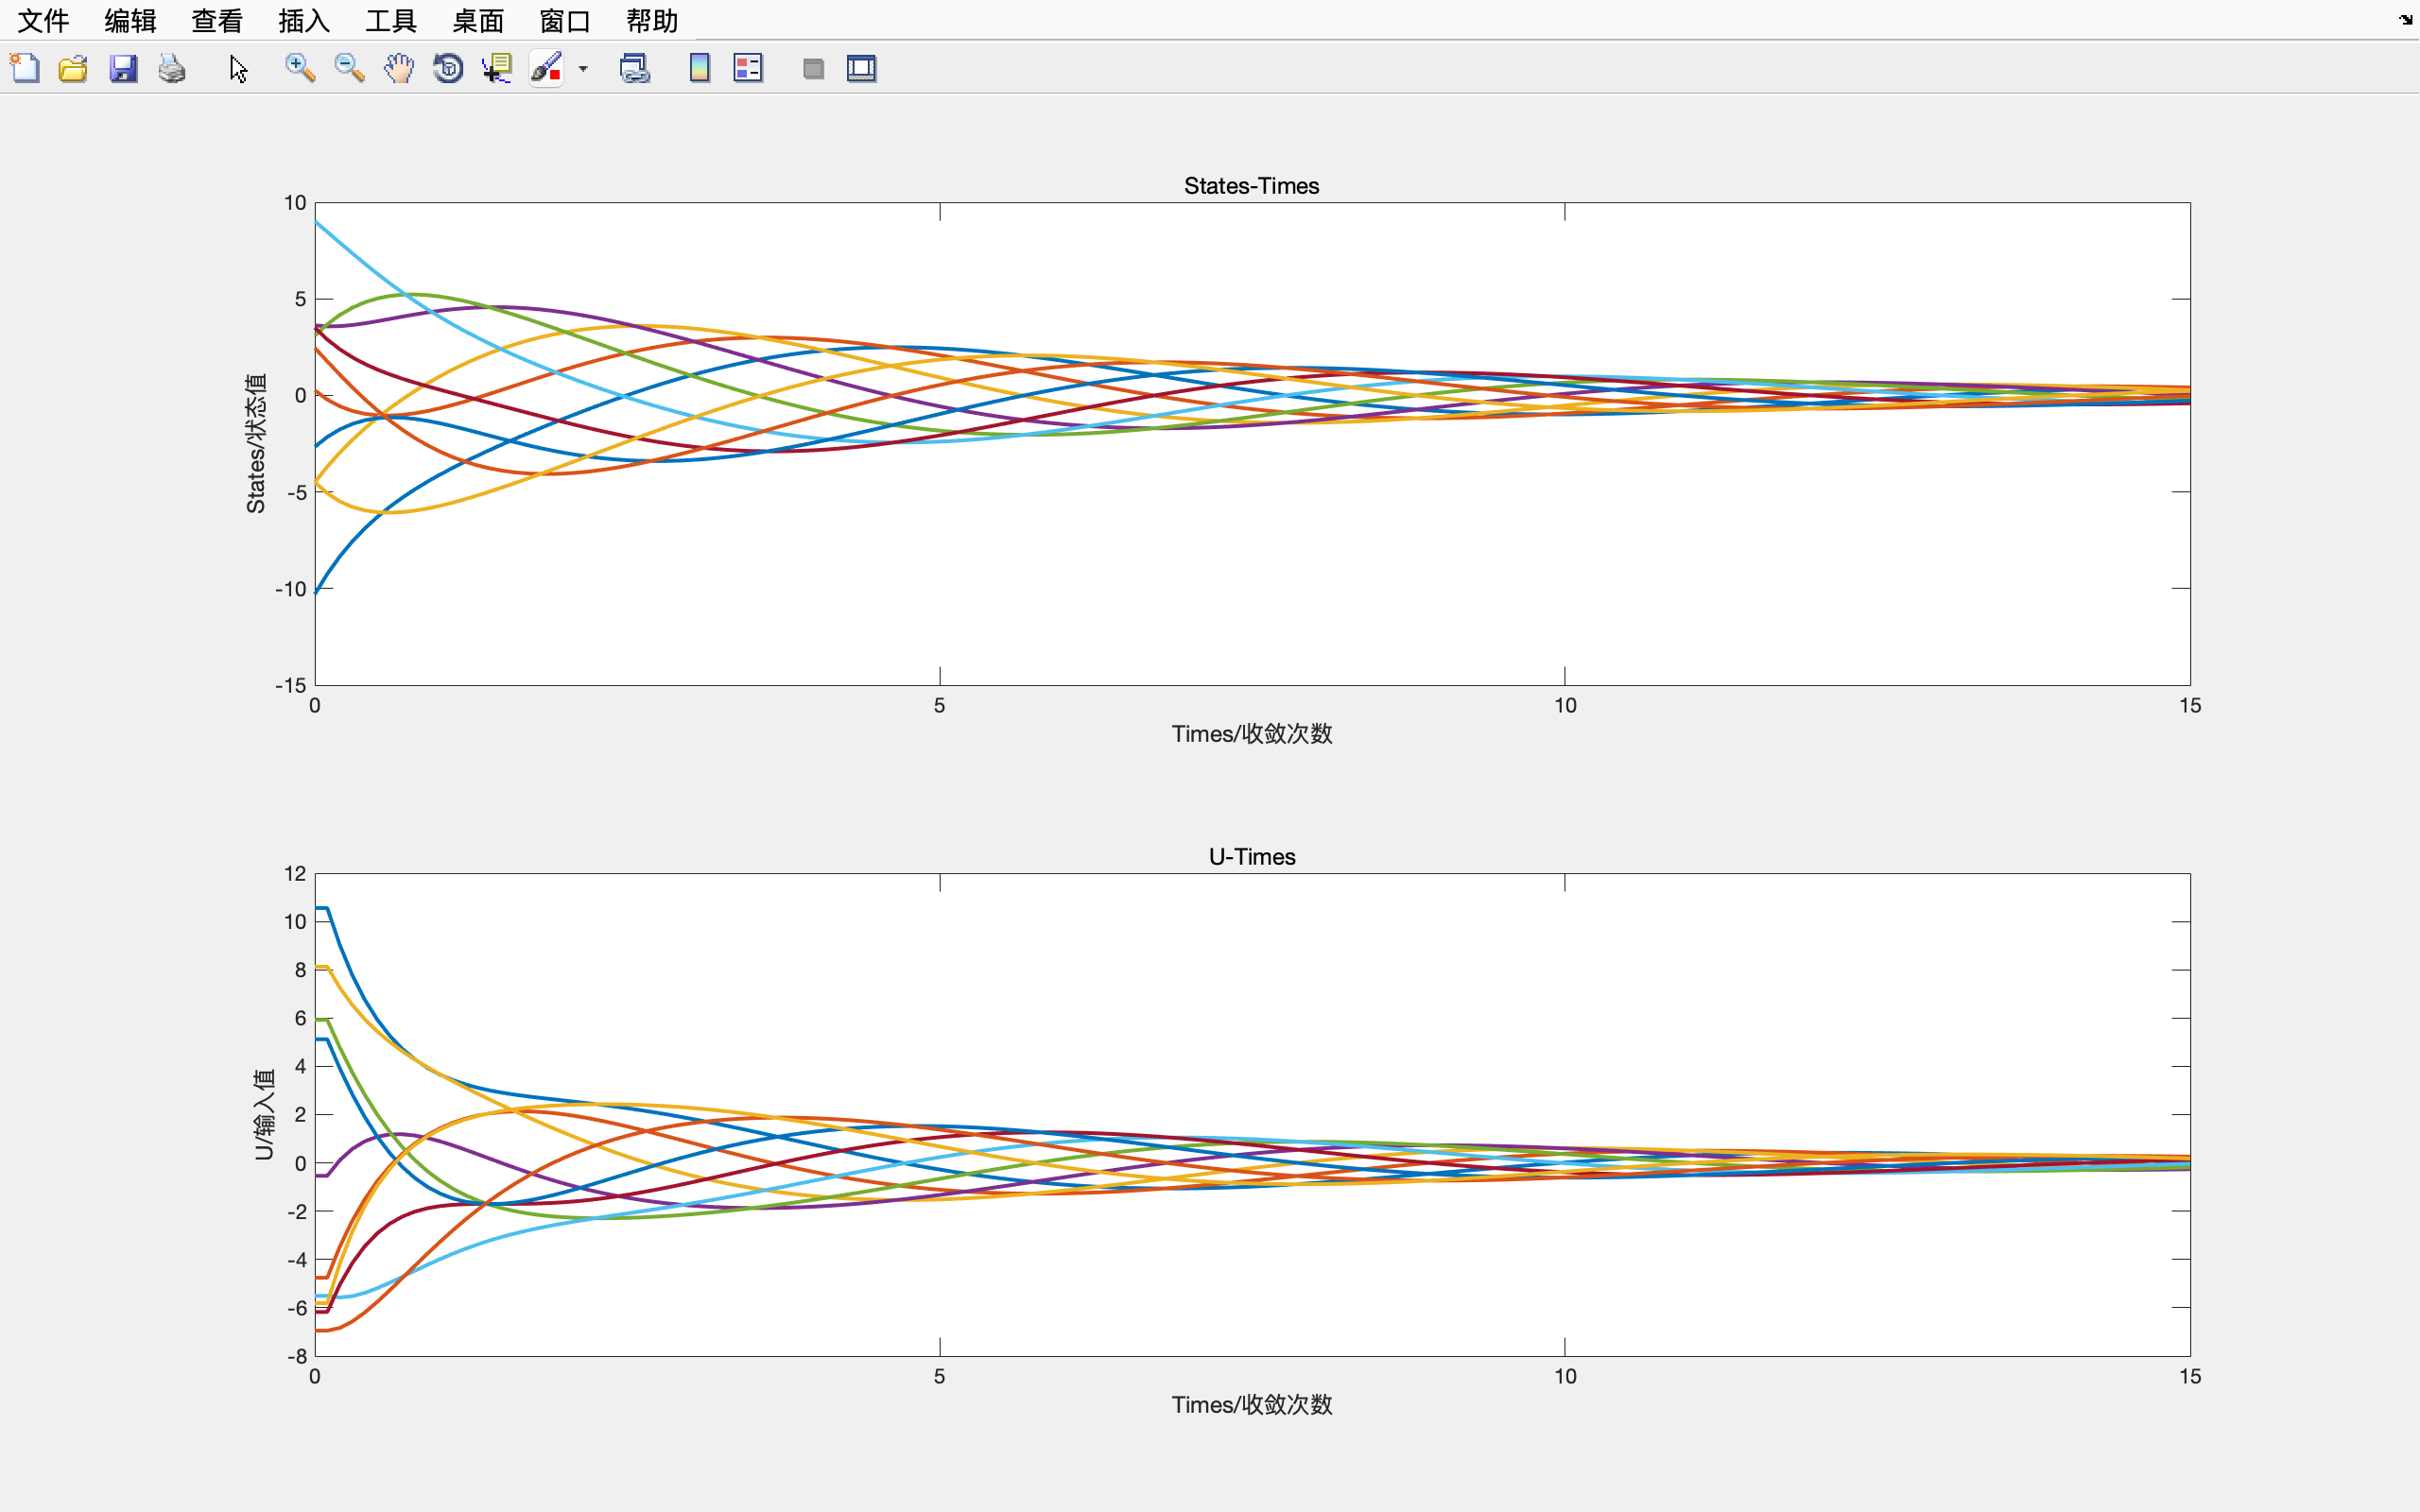
\includegraphics[width=12cm]{figures/Result1-Fig5a.png}
\end{figure}

\end{frame}
%---------------------------------------------------------
\begin{frame}
\frametitle{Simulation}
\begin{figure}[htbp]
    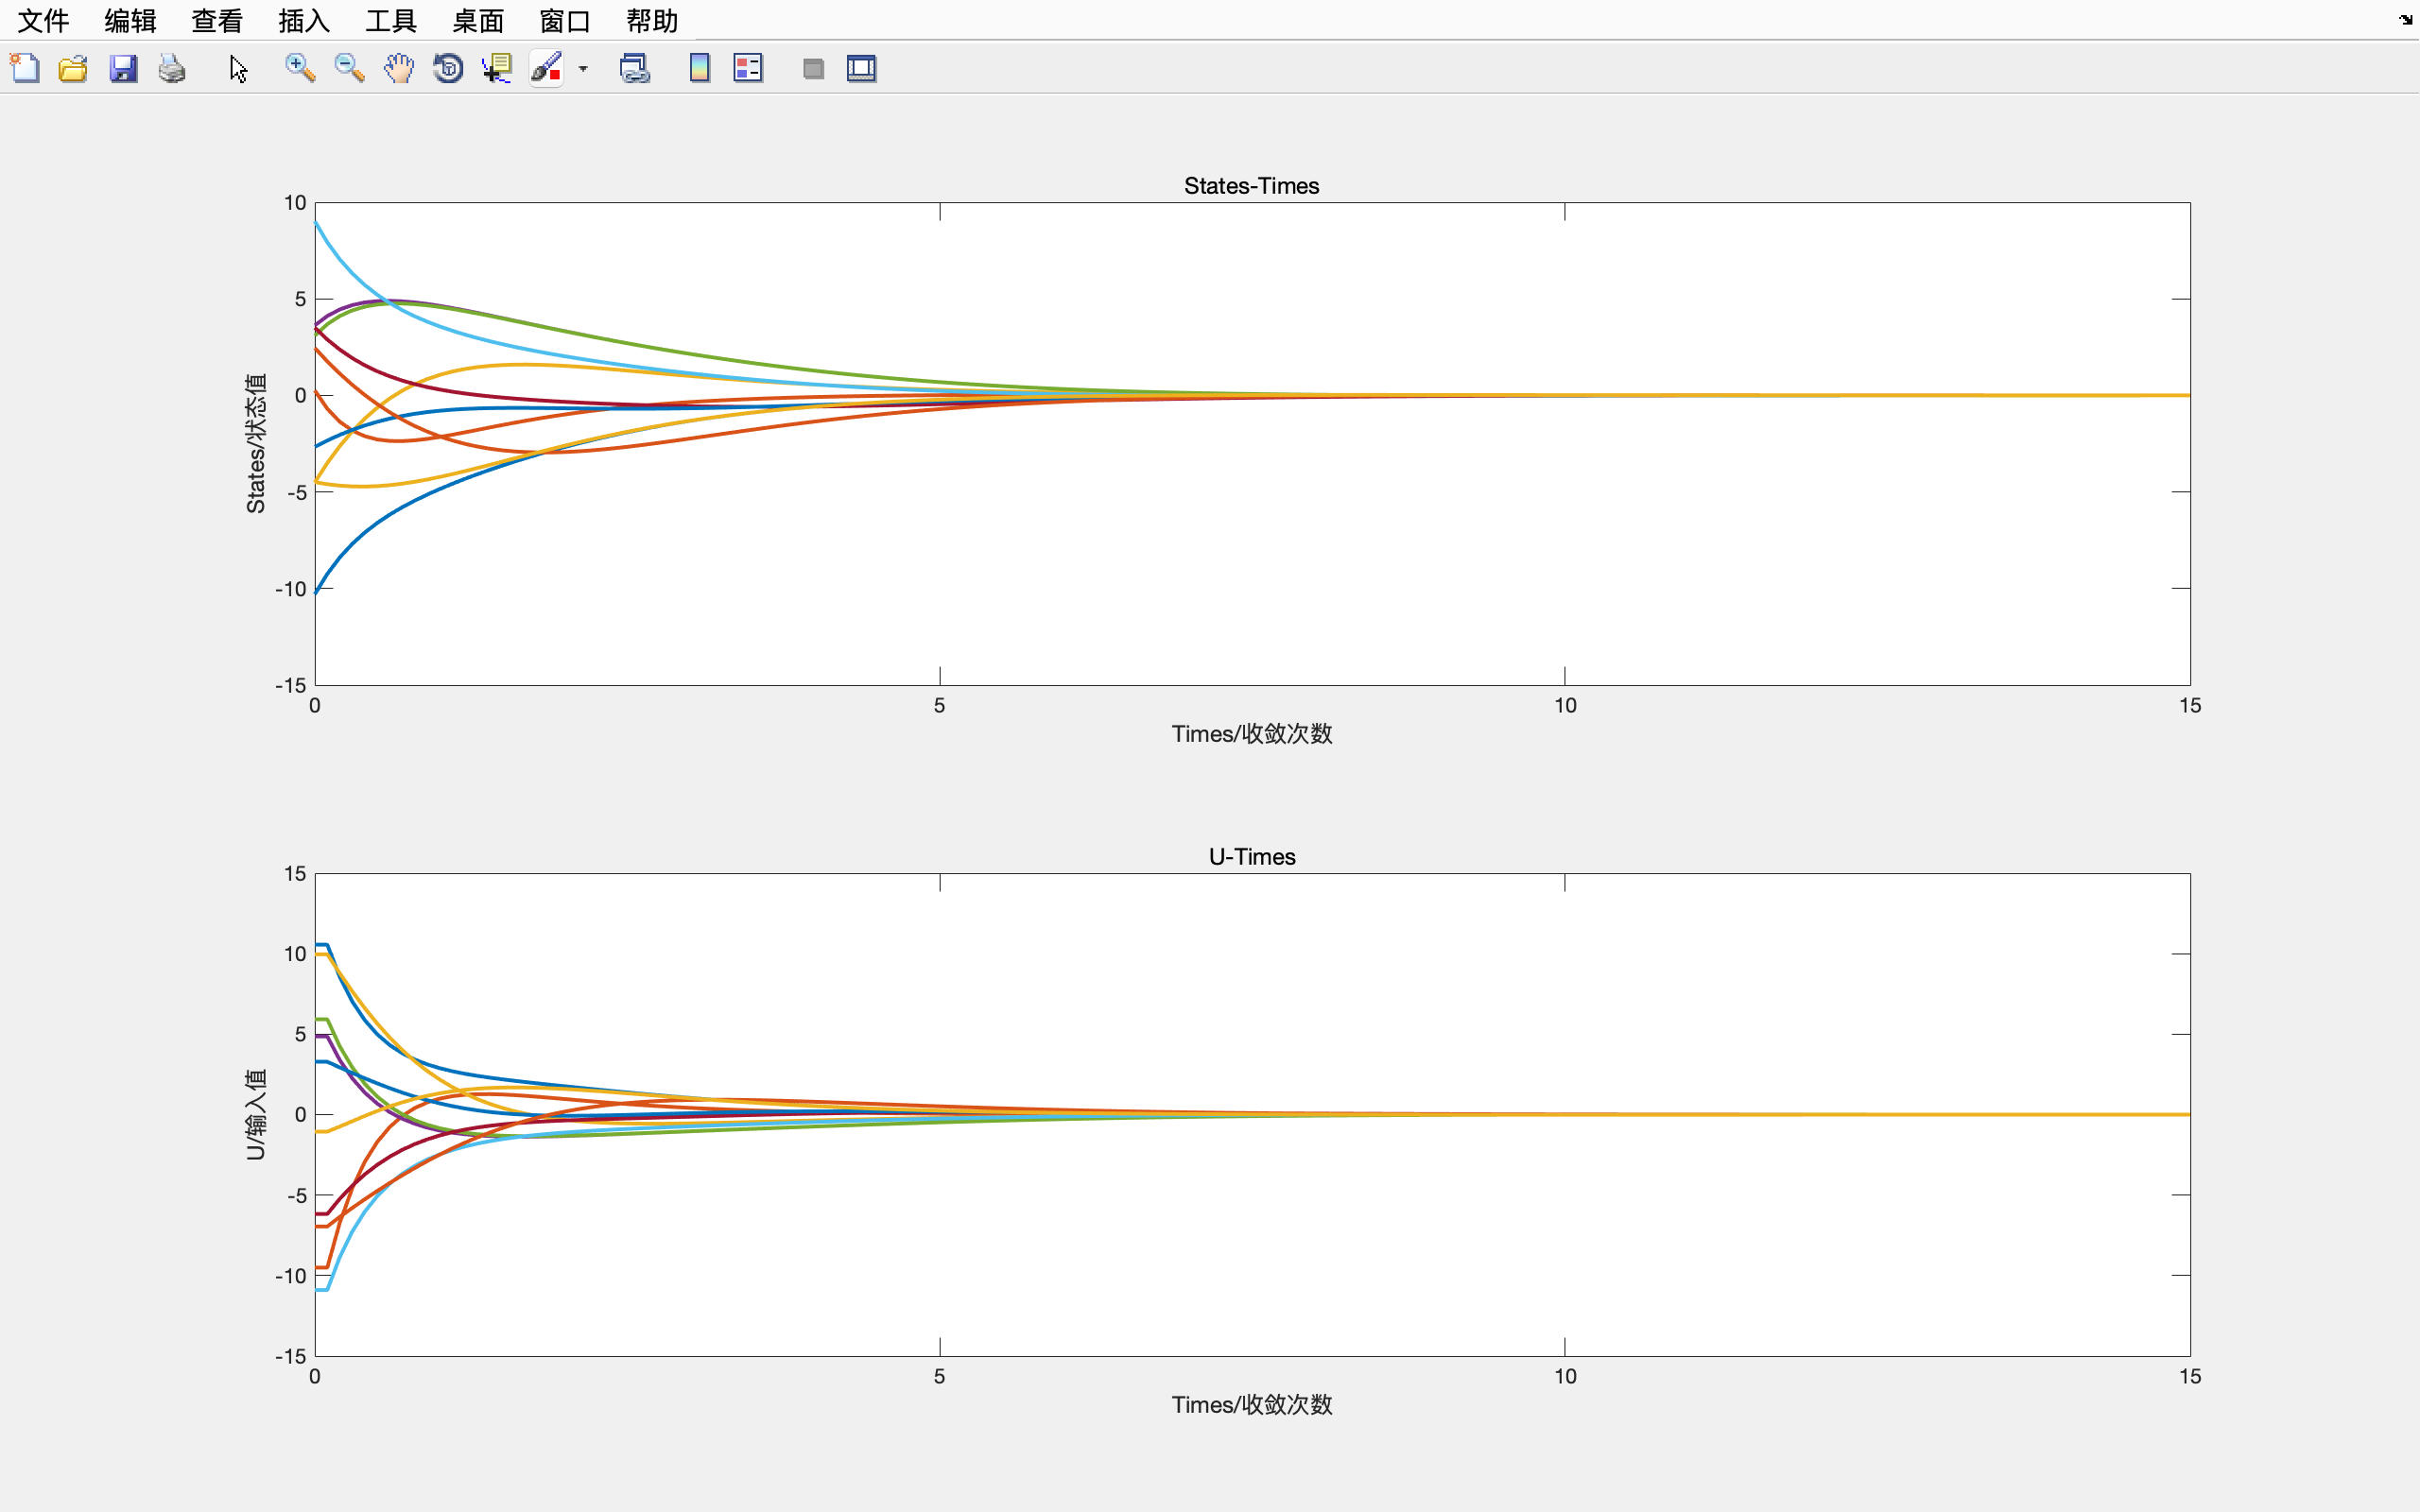
\includegraphics[width=12cm]{figures/Result2-Fig5b.png}
\end{figure}

\end{frame}
%---------------------------------------------------------
\begin{frame}
\frametitle{Simulation}
\begin{figure}[htbp]
    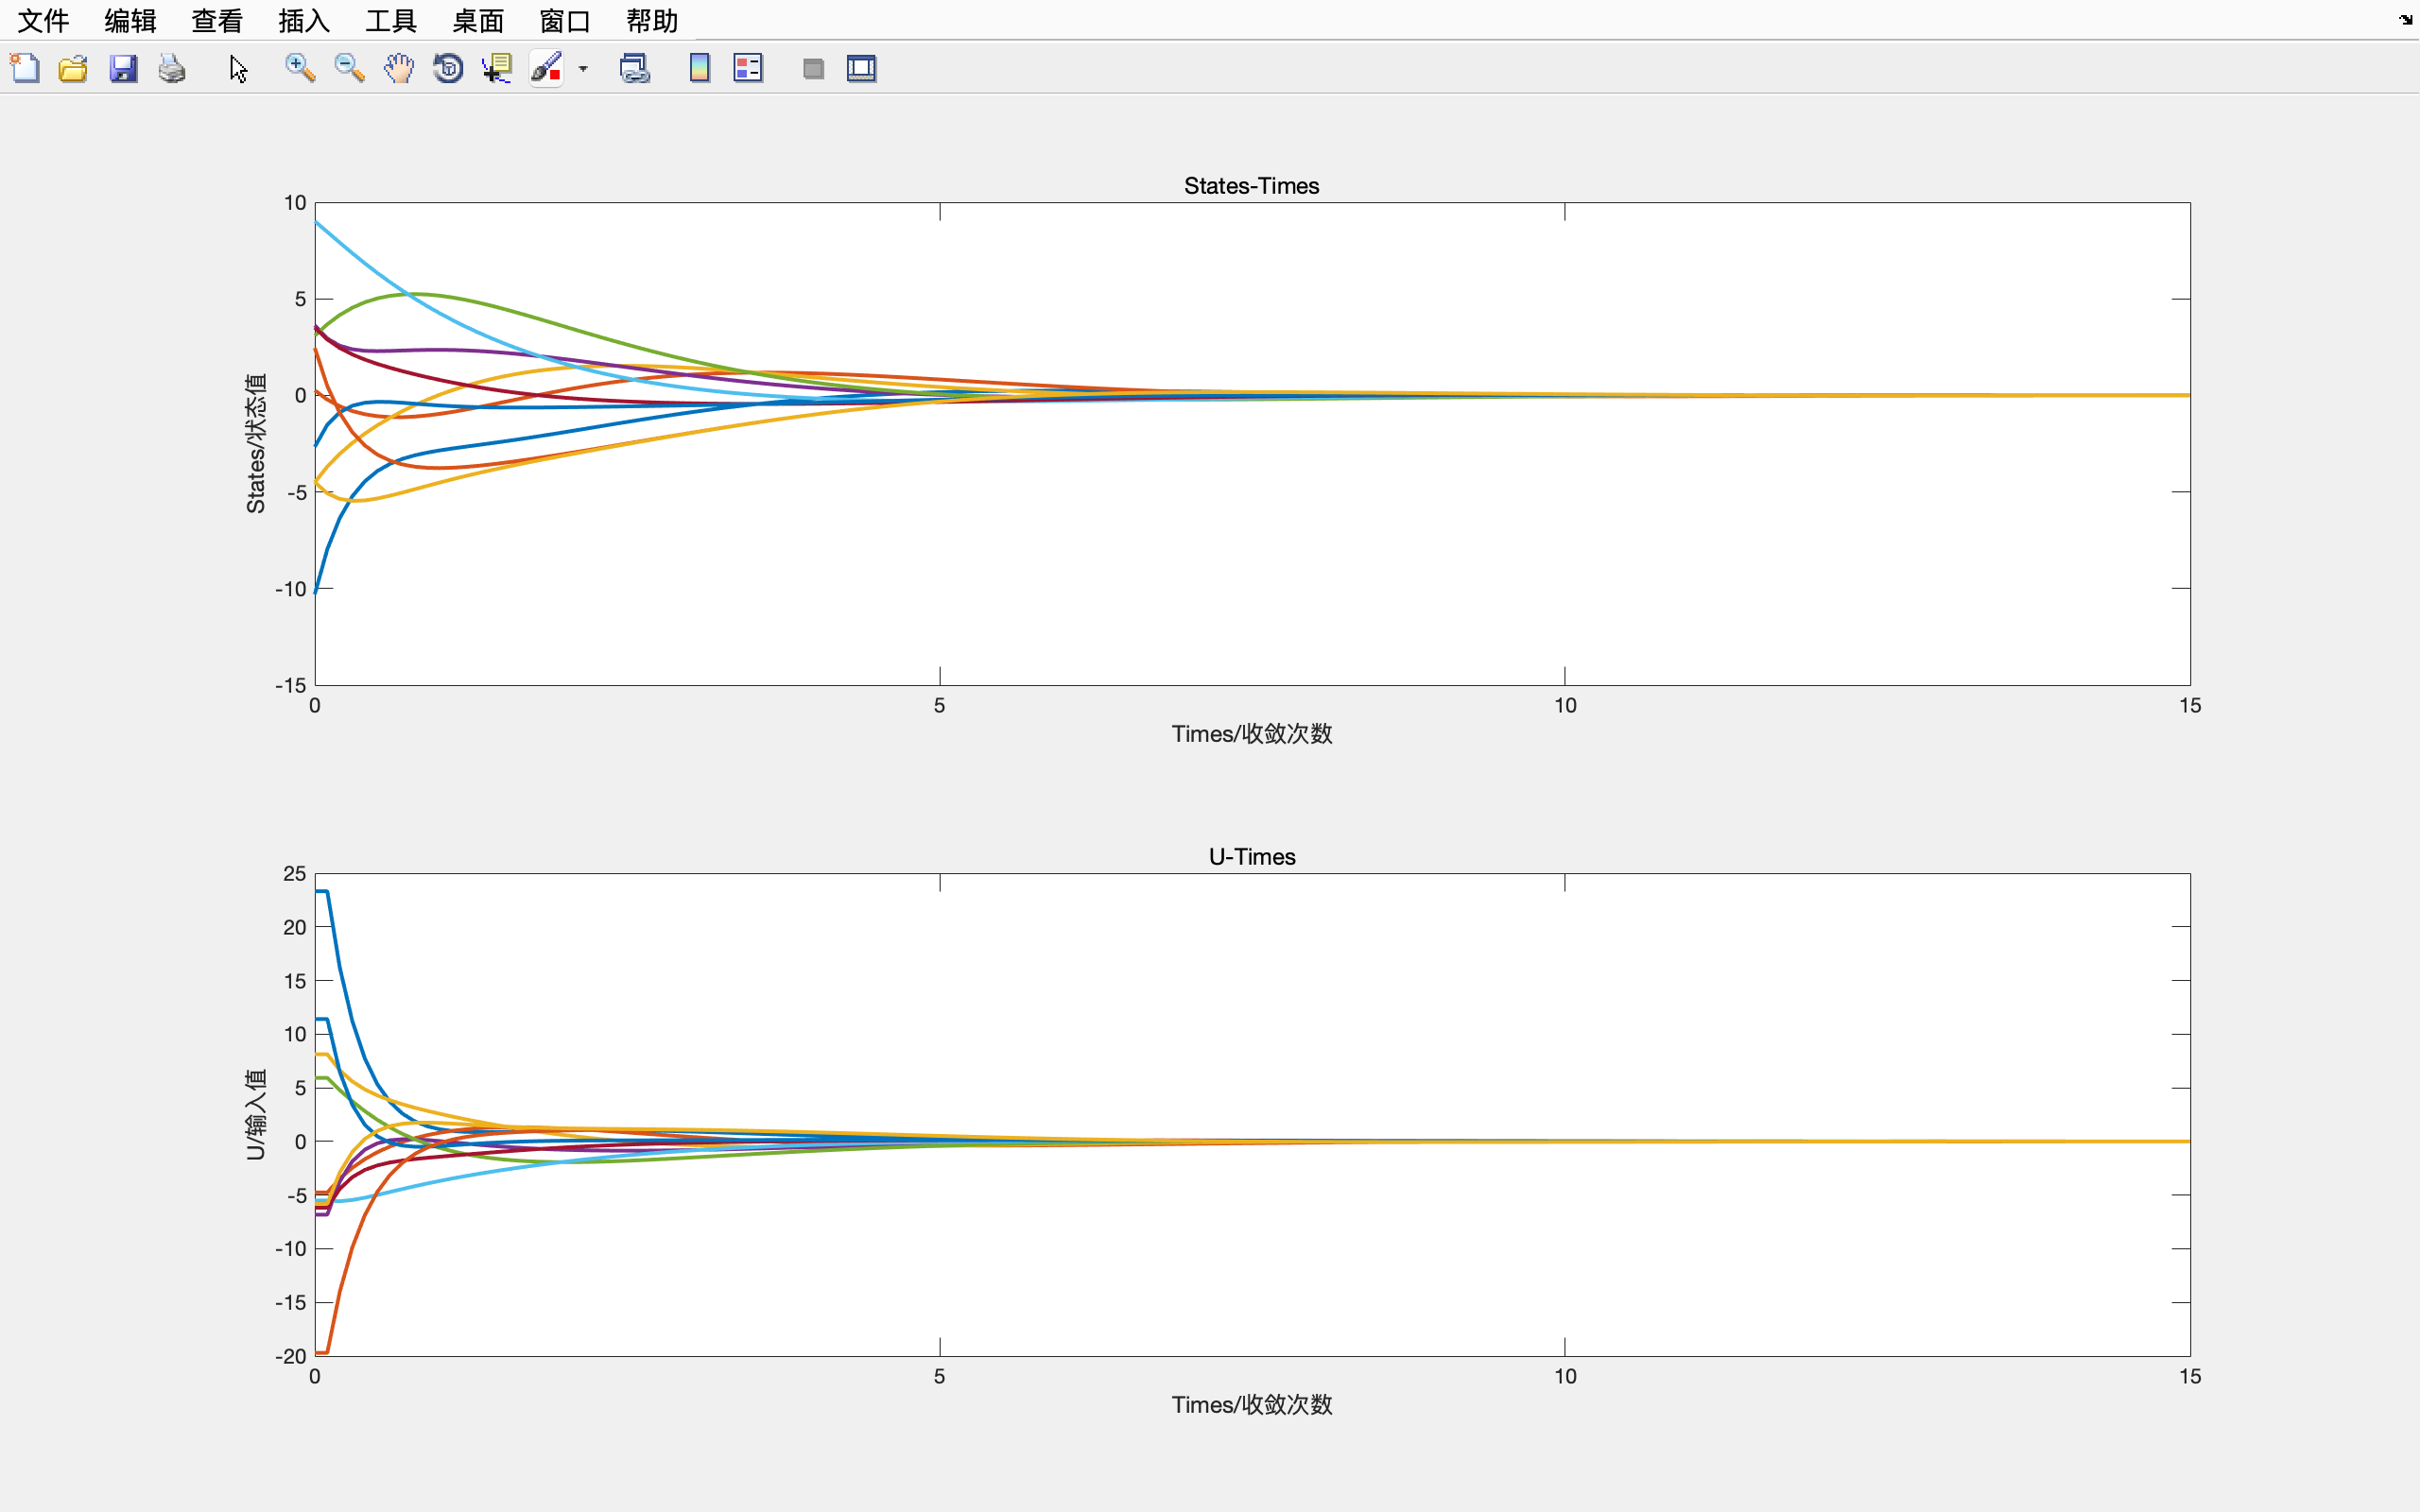
\includegraphics[width=12cm]{figures/Result3-Fig5c.png}
\end{figure}

\end{frame}
%---------------------------------------------------------
\begin{frame}
\frametitle{Simulation}
\begin{figure}[htbp]
    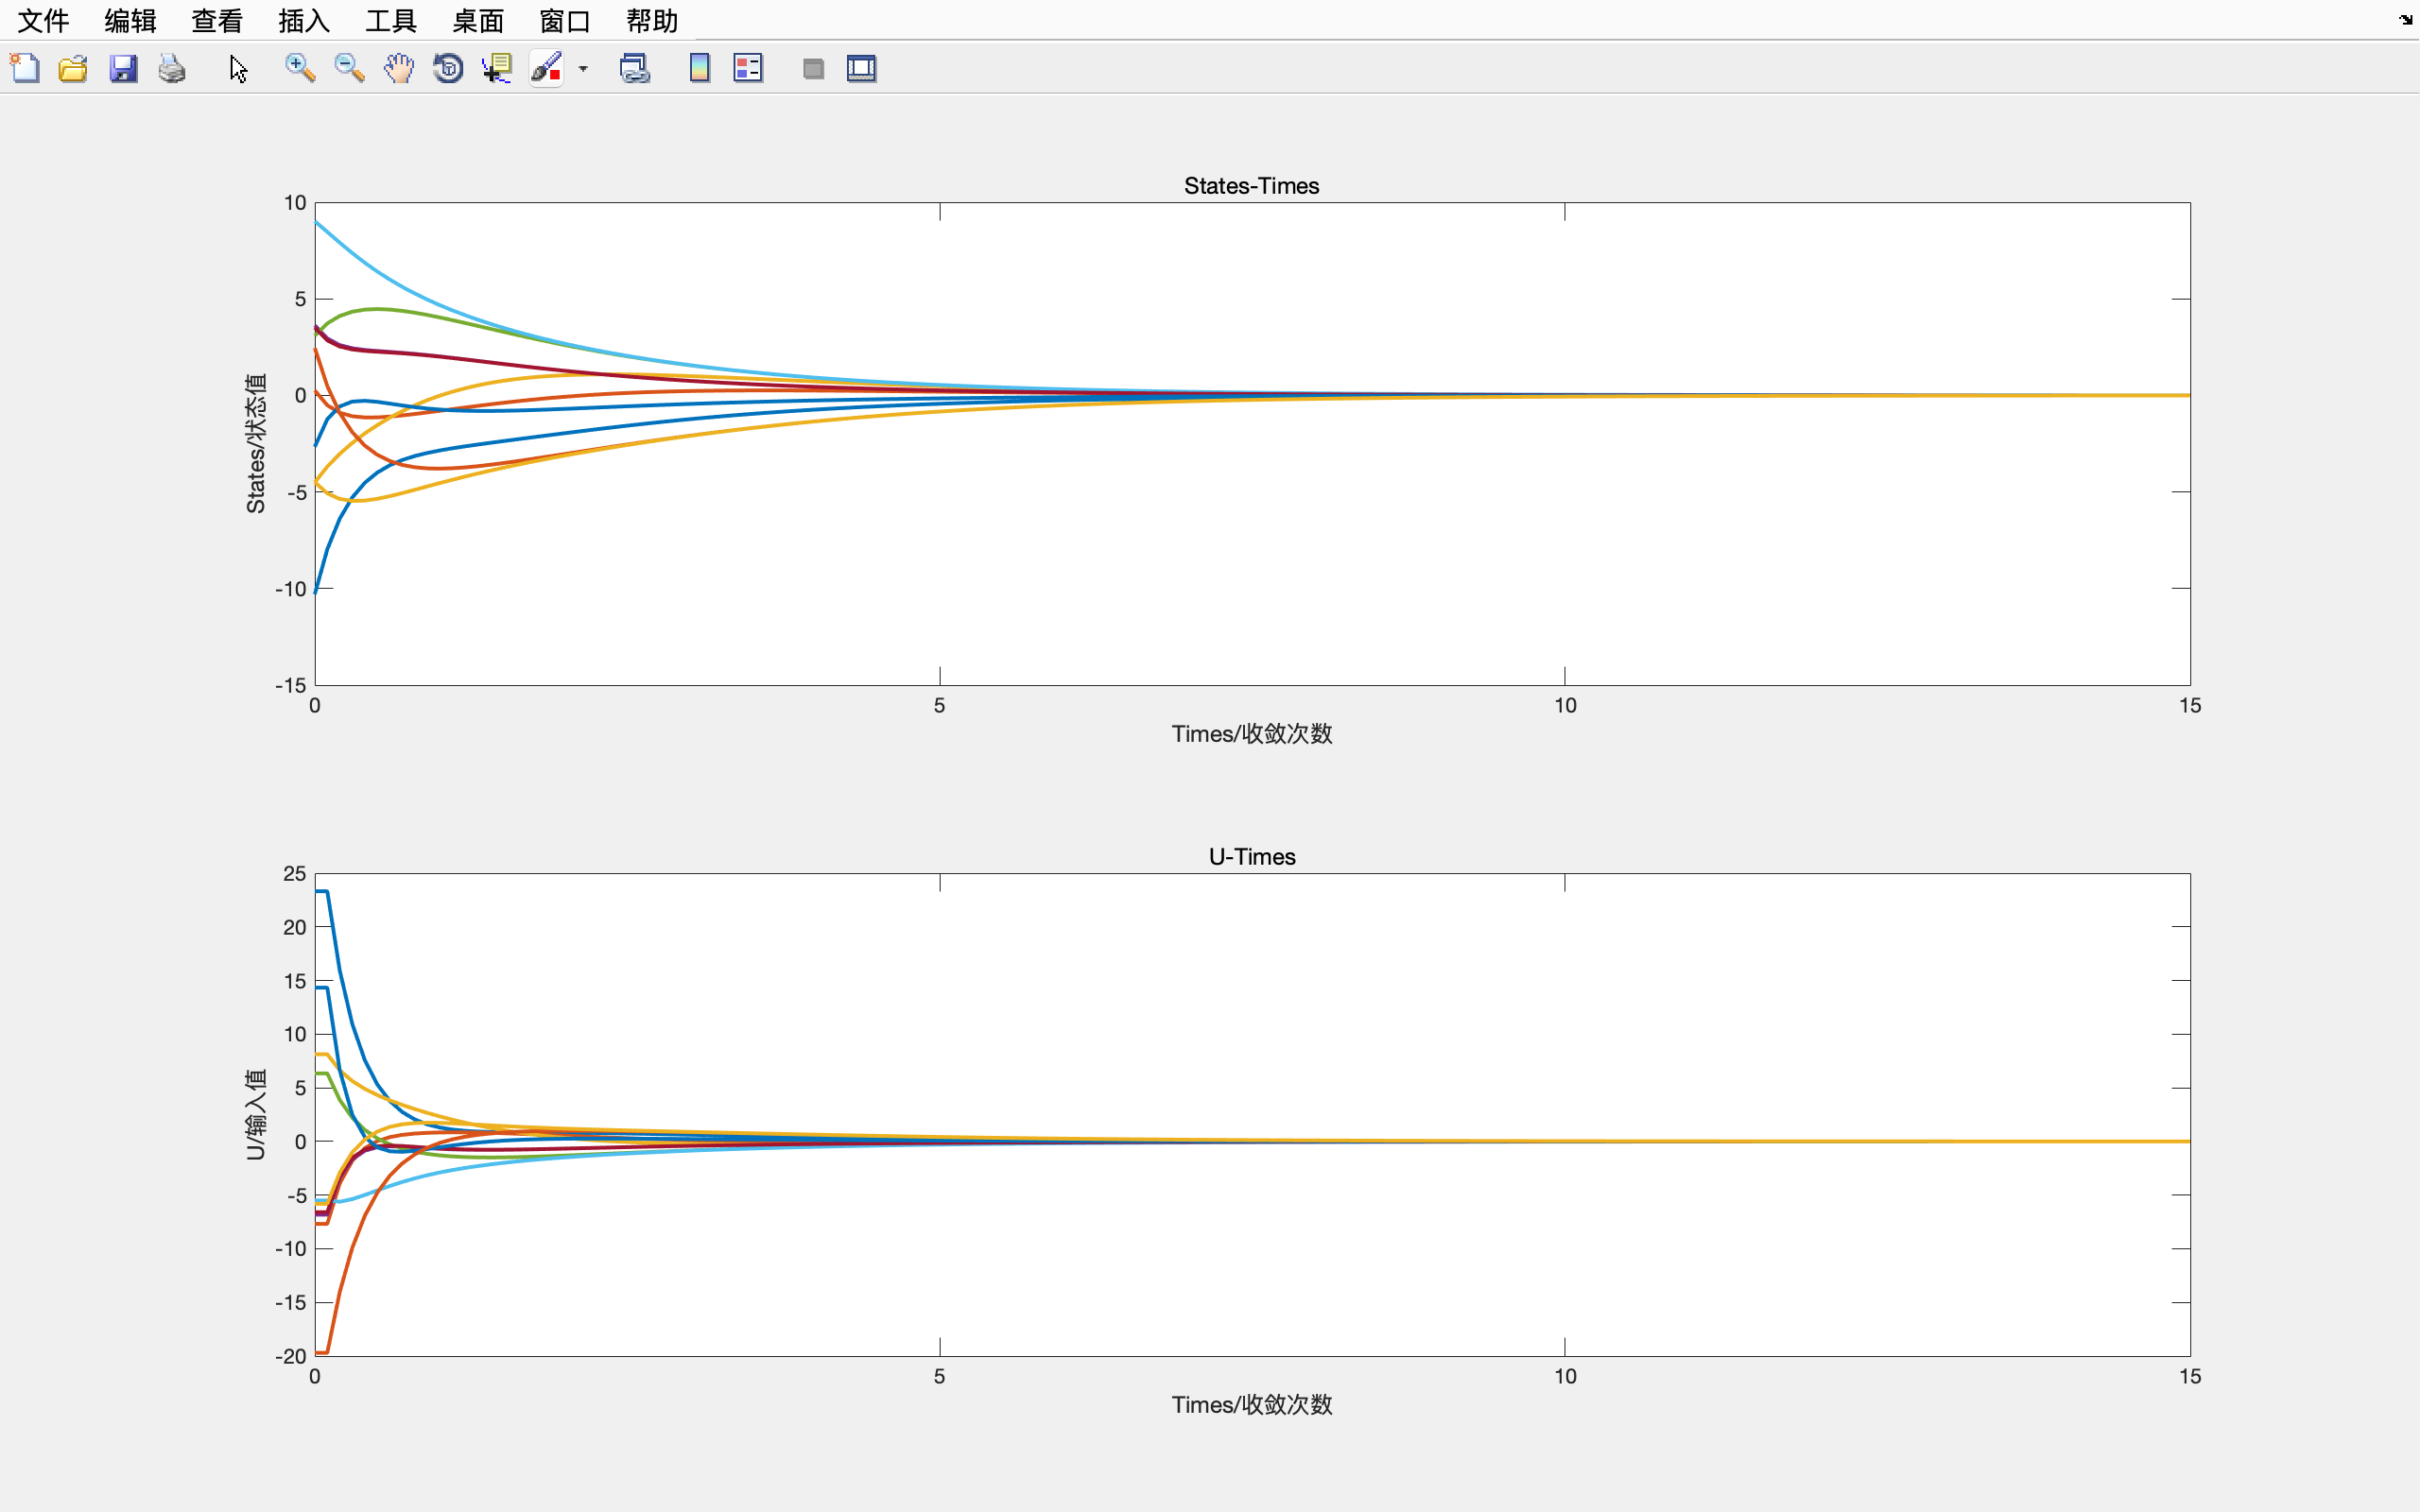
\includegraphics[width=12cm]{figures/Result4-Fig5d.png}
\end{figure}

\end{frame}
%---------------------------------------------------------

\end{document}